%!TEX root = ../thesis.tex
%*******************************************************************************
%*********************************** First Chapter *****************************
%*******************************************************************************

\chapter{Introduction \label{chap:1}}  %Title of the First Chapter

\ifpdf
    \graphicspath{{Chapter1/Figs/Raster/}{Chapter1/Figs/PDF/}{Chapter1/Figs/}{Chapter1/Figs/Vector/}}
\else
    \graphicspath{{Chapter1/Figs/Vector/}{Chapter1/Figs/}}
\fi



A new field of research in material science and condensed matter physics was formed after the synthesis of graphene in 2005 \cite{Novoselov666,Novoselov26072005}. This field is named Two-dimensional (2D) material due to the fact that graphene is a single atomic-layer crystal. The synthesis itself together with the phenomenal properties of graphene has leaded to a Nobel Price in physics rewarded to A. K. Geim and K. S. Novoselov \citep{Geim2007}. Since then, the field is expanding with the involvement of researcher not only from young community, but also from experts who have been working on materials like graphite, fullerenes and carbon nanotubes which are strongly graphene related. in the last five years While a part of these effects have been making to explore more on the graphene itself and its applications, some other parts were put on discovering new 2D materials. It has been evidenced from graphene, same material having different dimensionality can have different properties. Therefore, many materials with hidden properties which will only manifest itself at other dimensions yet to be discovered. 

\begin{figure}[htbp!] 
\centering    
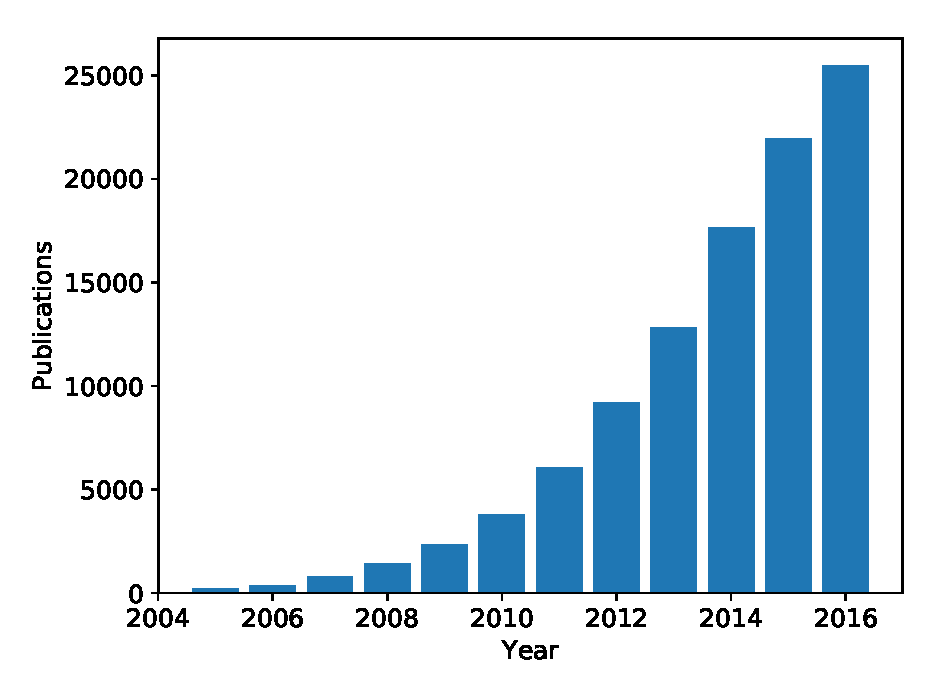
\includegraphics[width=0.7\textwidth]{graphene_papers.eps}
\caption{Graphene related publication during the last decade. Source ISI Web of Science.} \footnote{This result is obtained by searching for "graphene" in the topic field} 
\label{fig:grpapers}
\end{figure}

\mynote{make the footnote work, and save the python code for plotting}

On the other hand, with the advent of powerful supercomputer facilities, calculations that seems impossible to finish in a reasonable time now has been made accessible. At the same time, given the accuracy of the calculations is the most crucial aspect of computational physics, especially when the results are related to the prediction the real properties of materials, researchers and programmers have been making important progress to make sure theories and its implementation are correct and the results they yield are within acceptable precision. Equipped with these tools, theoretical predictions on the structure and the properties of material have served well on discovering unexplored features. Moreover, detailed characterizations at atomic scale benefits the experimental results to make it more convincing, or even sometimes to explain the unexpected results.

Considering all mentioned, it is a sound approach to apply the state-of-the-art computational methods that accompanied with high-performance supercomputer facilities to investigate the physical properties of novel 2D materials. This thesis is a summary of several works which has accomplished during my PhD study and were initiated to this end. The thesis is organized as followed: For the rest of this chapter, I will first introduce graphene and some post-graphene materials that discovered right after graphene and, briefly, methods used to synthesis 2D materials. The following \autoref{chap:2} will present the computational methods, the theory behind and the implementations of them. In \autoref{chap:3}, I will discuss several general properties of 2D materials. The next two chapters will be the main results from my works. Starting from specific properties targeting at specific novel 2D materails in \autoref{chap:4}, and followed by modification of physical properties of 2D materials in \autoref{chap:5}. Conclusions for the thesis will be given in the last chapter.

\section{Graphene}
\subsection{History and prediction}
\subsection{Physical properties}
\section{Post-graphene Materials}
\subsection{Functionized Graphene}
\subsubsection{Graphane}
\subsubsection{Fluorographene}
\subsection{Boron Nitride}
\subsection{Silicene and Germanene}
\subsection{Transition Metal Dichalcogenides}
\section{0D and 1D from 2D: buckyballs, nanotubes and nanoribbons}
\section{Synthesis methods}
